%==========================================================
%   Modern Informatics Research Review LaTeX Template
%==========================================================

\documentclass[a4paper,11pt]{article}

%-------------------- Packages ----------------------------
\usepackage[utf8]{inputenc}        % UTF-8 encoding
\usepackage[T1]{fontenc}           % Font encoding
\usepackage{lmodern}               % Clean, scalable fonts
\usepackage[pdftex]{graphicx}      % Graphics support
\usepackage{url}                    % Better URL handling
\usepackage{datetime}               % Custom date formatting
\usepackage{pgfgantt}               % Gantt charts
\usepackage{xcolor}                 % Color definitions
\usepackage{geometry}               % Page margins
\usepackage{fancyhdr}               % Headers and footers
\usepackage{titlesec}               % Custom section titles
\usepackage{booktabs}               % Cleaner tables
\usepackage{float}               

%-------------------- Page Setup --------------------------
\geometry{a4paper, left=25mm, right=25mm, top=25mm, bottom=25mm}
\parindent=0pt                      % No paragraph indentation
\parskip=6pt                        % Space between paragraphs
\Urlmuskip=0mu plus 1mu             % Better URL line breaks

%-------------------- Colors -----------------------------
\definecolor{mainblue}{RGB}{51,102,204}
\definecolor{accentblue}{RGB}{153,204,254}

%-------------------- Date Format -------------------------
\newdateformat{monthyeardate}{\monthname[\THEMONTH] \THEYEAR}

%-------------------- Header & Footer --------------------
\pagestyle{fancy}
\fancyhf{}
\lhead{\textbf{MSc Informatics Project Progress Report}}
\rhead{\thepage}
\lfoot{\small School of Informatics}
\rfoot{\monthyeardate\today}
\renewcommand{\headrulewidth}{1pt}
\renewcommand{\footrulewidth}{0.5pt}

%-------------------- Section Styles ----------------------
\titleformat{\section}{\Large\bfseries\color{mainblue}}{\thesection.}{1em}{}
\titleformat{\subsection}{\large\bfseries\color{mainblue}}{\thesubsection.}{1em}{}

%-------------------- Title Page Info ---------------------
\newcommand{\examnumber}{B299013}
\newcommand{\field}{Small Language Models for AI-Generated Text Detection: An Ablation Study on Curvature Methods}
\newcommand{\tutor}{Dr. Rik Sarkar}
\newcommand{\supervisor}{Dr. Rik Sarkar}

%==========================================================
\begin{document}

%-------------------- Title Page --------------------------
\begin{titlepage}
\begin{center}
\vspace*{2cm}

\includegraphics[width=40mm]{crest.png}\\[1cm]

{\Huge\bf School of Informatics}\\[1.5cm]

{\LARGE\bf MSc Informatics Project Progress Report}\\[0.5cm]
{\Large\bf \field}\\[2cm]

{\large \textbf{UID:} \examnumber}\\[0.5cm]
{\large \textbf{Date:} \monthyeardate\today}\\[2cm]

{\large \textbf{Tutor:} \tutor\\[0.2cm]
\textbf{Supervisor:} \supervisor}
\vfill
\end{center}
% Please delete as appropriate for you (give or do not give)
\textit{I give /do not give permission for future Informatics Project Proposal classes to read an anonymous version of this document.}

\textit{This page does not count towards the page limit.}
\end{titlepage}



\section{Goal of the Project}
The primary goal of this project is to conduct a comprehensive ablation study on the components of curvature-based (loss landscape) AI-generated text detection, with a particular focus on the efficacy of small language models. This project aims to isolate and analyse the specific variables that drive detection efficacy by systematically removing or altering key components of the detection pipeline. 

The research investigates whether model scale, training duration, and perturbation strategies significantly influence the ability to distinguish between human-written and machine-generated text. Therefore, this project is structured around four core experimental objectives:

\begin{enumerate}
    \item \textbf{Experiment 1 (Cross-Detection and Model Scale):} Investigate the relationship between detector model size and detection performance by mapping the cross-detection interactions across varying scales of generative and detector models to establish a foundation for the ablation study.
    \item \textbf{Experiment 2 (Training Dynamics):} Analyse how detector training duration, measured in checkpoint steps, impacts detection efficacy and identify optimal training thresholds before overfitting occurs.
    \item \textbf{Experiment 3 (Semantic Perturbation Scale):} Evaluate the impact of the mask-filling model's capacity on detection accuracy by comparing different sizes of the T5 model (T5-small, T5-large, and T5-3B) to determine if the standard T5-large model is sufficient or if larger models are strictly necessary.
    \item \textbf{Experiment 4 (Evaluation of Perturbation Strategies):} Conduct a systematic evaluation of different perturbation strategies (ranging from high-semantic text to pure noise) to determine the minimum linguistic and statistical requirements for the curvature metric to function effectively.
\end{enumerate}

\section{Methods}
The project employs a systematic, quantitative experimental design utilising a standardized evaluation framework. The core metric for evaluation across all experiments is the Area Under the Receiver Operating Characteristic Curve (AUROC), which measures the detector's ability to distinguish human-written text from machine-generated text. The evaluation dataset for all experiments is sourced from the WritingPrompts dataset, consisting of a balanced target pool of 250 human-written samples and 250 machine-generated samples.

The methodology is divided into the four distinct experimental tests outlined above, manipulating three primary variables:

\begin{itemize}
    \item \textbf{Model Scale and Architecture (Experiment 1):} Evaluating cross-model and self-model generation using a diverse suite of Generators (e.g., GPT-2, OPT, SmolLM) and Detectors (e.g., Pythia) ranging from 70M to 1.7B parameters. This specifically tests whether smaller detector models demonstrate superior performance across a broader range of generator architectures compared to larger detectors.
    \item \textbf{Training Dynamics (Experiment 2):} Tracking detector performance across various training checkpoints (from 1k to 143k steps) to observe the evolution of detection capabilities over time, specifically testing whether partially trained models exhibit different detection characteristics compared to fully trained checkpoints.
    \item \textbf{Semantic Perturbation Scale (Experiment 3):} Comparing the efficacy of different T5 model sizes (T5-small, T5-large, and T5-3B) as the mask-filling model. This tests how the parameter count of the semantic perturbation model impacts the quality of the generated neighbouring texts and the resulting curvature metric, with T5-large serving as the standard configuration.
    \item \textbf{Evaluation of Perturbation Strategies (Experiment 4):} Systematically altering the perturbation strategy to test the detector's reliance on specific linguistic features. This creates four distinct tests to evaluate how the nature of the generated neighbours affects detection:
    \begin{enumerate}
        \item \textit{Control (T5-large Mask-Filling):} High semantics, syntax, and statistical plausibility.
        \item \textit{Test A (WordNet Synonyms):} High semantics and statistical plausibility, but broken syntax.
        \item \textit{Test B (Unigram Frequency):} Zero semantics, zero syntax, but high statistical plausibility (real English words).
        \item \textit{Test C (Random Tokens):} Pure noise or gibberish (subword token noise).
    \end{enumerate}
\end{itemize}

Data analysis and visualisation were conducted to aggregate the experimental results and evaluate detection efficacy across the different variables.

\section{What Has Been Accomplished So Far}
Significant progress has been made in completing the foundational experiments (Experiments 1 and 2):

\textbf{Experiment 1: Cross-Detection and Model Scale (Completed).} 
I successfully evaluated the interaction between generator and detector model scales to investigate whether smaller language models demonstrate superior detection capabilities. By running a comprehensive cross-evaluation, I generated a performance matrix sorted from largest to smallest parameter count. This experiment established the initial AUROC scores and confirmed the theoretical expectations: smaller detector models tend to achieve higher detection performance across diverse generator architectures, while larger detectors show more conservative likelihood assignments that limit their cross-detection effectiveness.

\begin{figure}[H]
    \centering
    % UPDATE THE FILENAME BELOW TO MATCH YOUR ACTUAL IMAGE FILE
    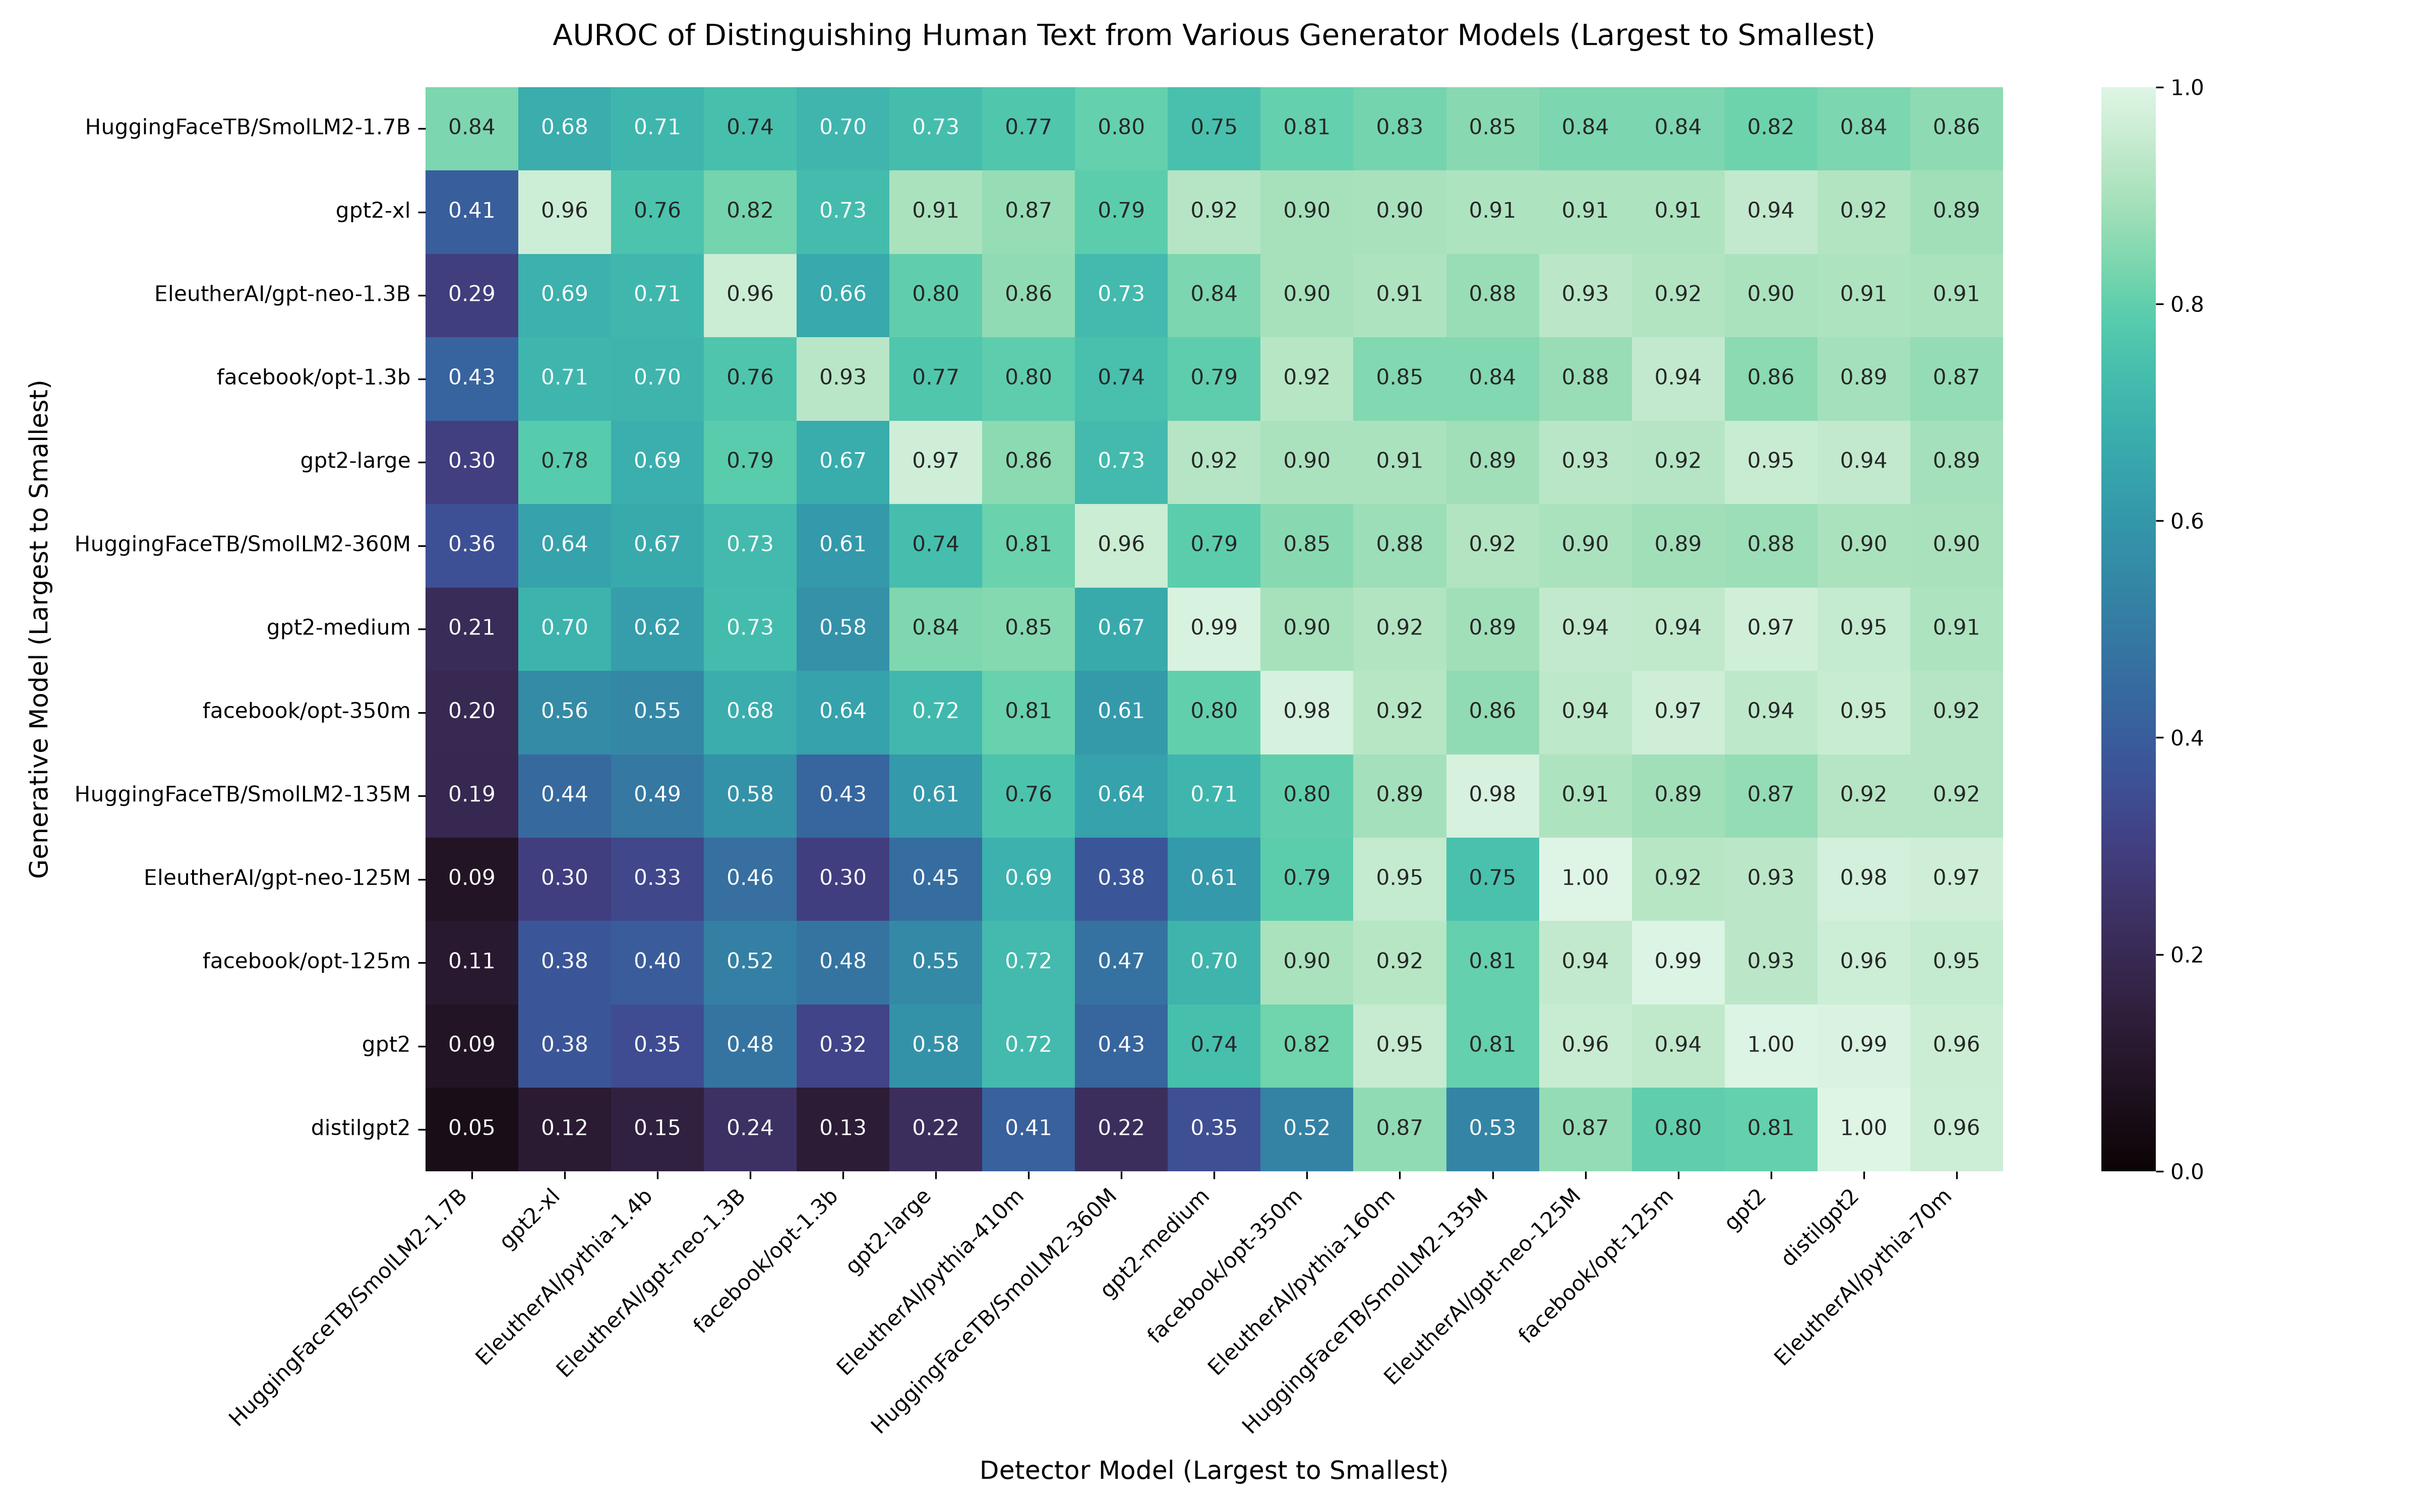
\includegraphics[width=0.55\textwidth]{cross_heatmap_matrix.png} 
    \caption{AUROC of distinguishing human text from various generator models. Rows represent generative models and columns represent detector models, both sorted from largest to smallest parameter count.}
    \label{fig:exp1_heatmap}
\end{figure}

\textbf{Experiment 2: Detector Training Steps (Completed).} 
I analysed how the AUROC evolves as the detector model trains. I extracted and organised the performance metrics across various training checkpoints (e.g., 1k, 50k, 143k). The resulting heatmaps map the detector model and step size against various generators. The results indicate that partially trained models (often around the 10k to 50k step mark) consistently outperform the fully trained 143k checkpoints, suggesting that earlier training checkpoints possess different likelihood surface characteristics that aid in cross-detection.

\begin{figure}[H]
    \centering
    % UPDATE THE FILENAME BELOW TO MATCH YOUR ACTUAL IMAGE FILE
    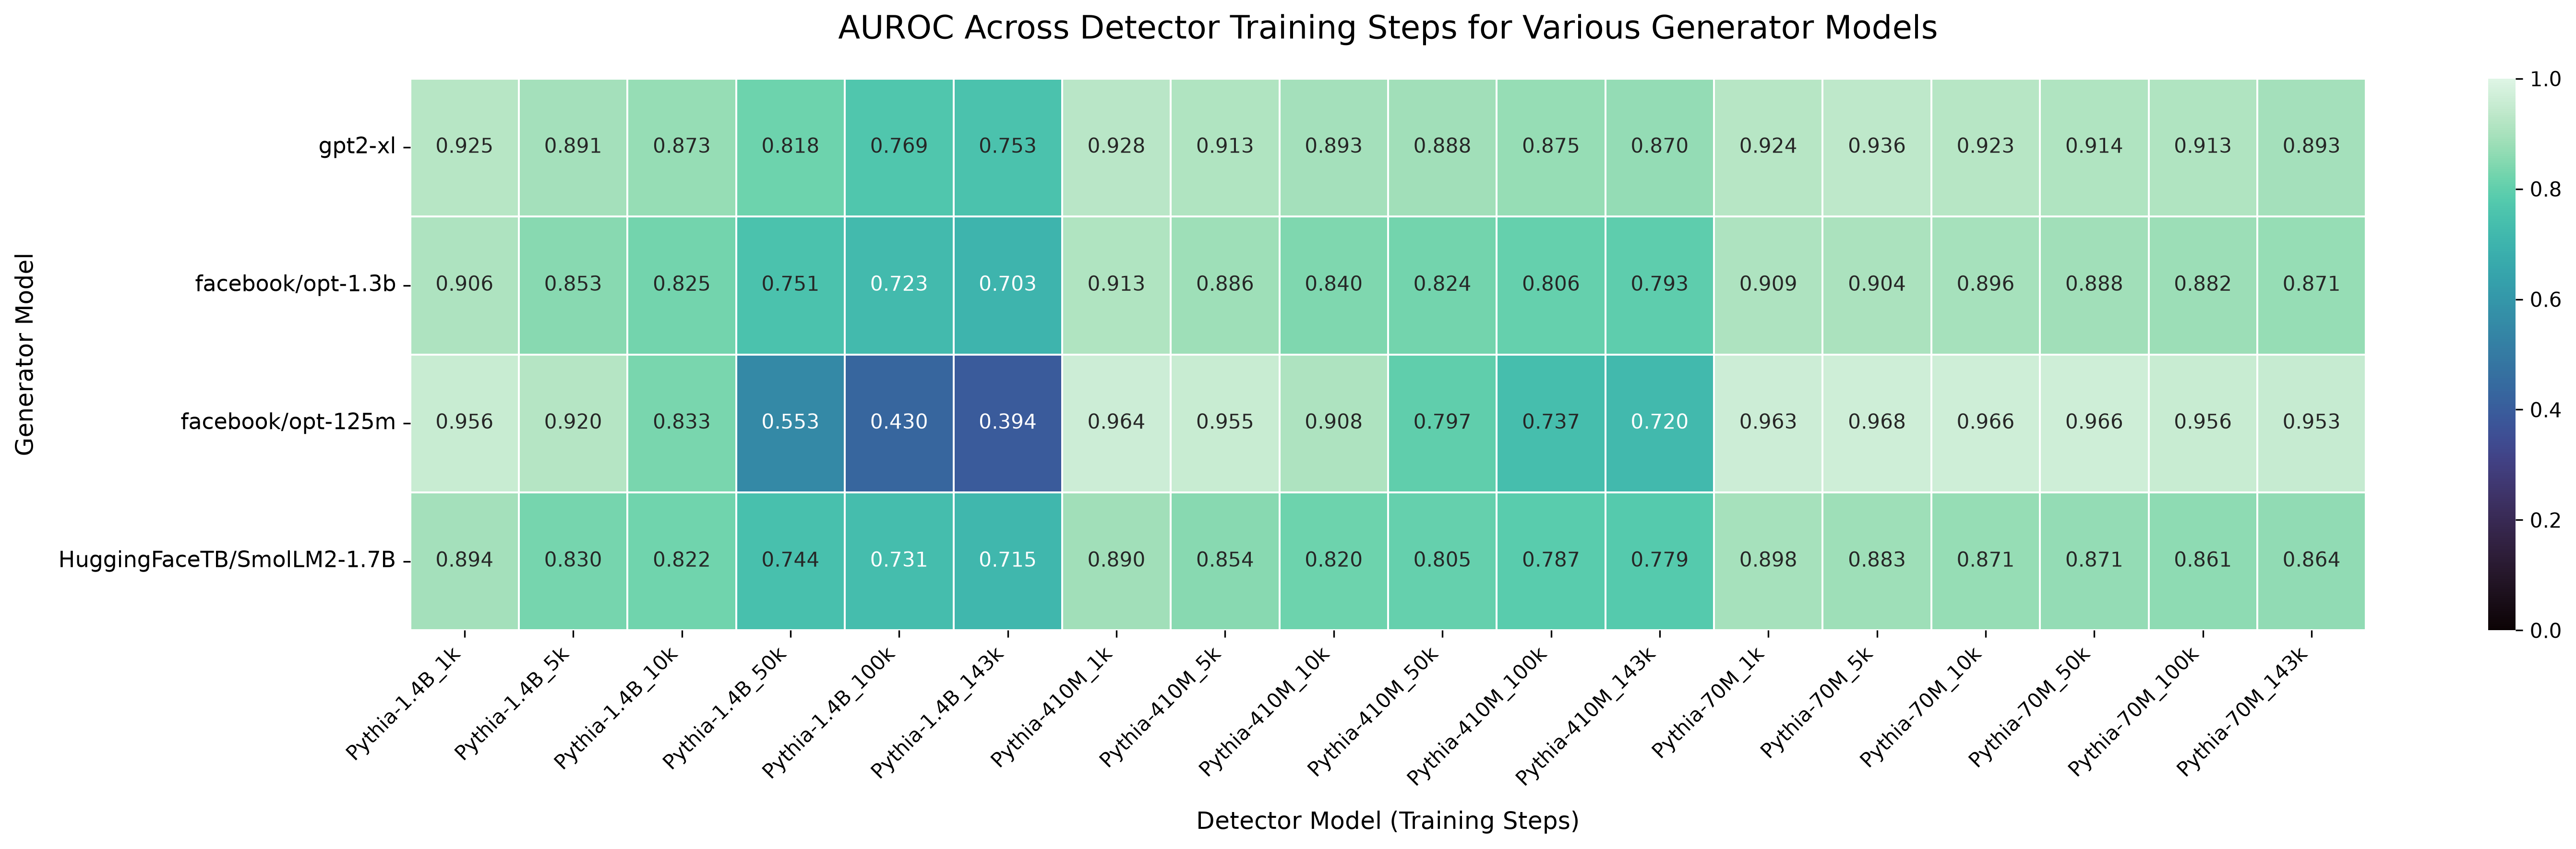
\includegraphics[width=0.75\textwidth]{stepsizes_combined_matrix.png}
    \caption{AUROC across detector training steps for various generator models. The x-axis combines the detector model and its training step checkpoint.}
    \label{fig:exp2_heatmap}
\end{figure}

\section{What Remains to be Done}
The remaining work focuses on the core theoretical contributions of the thesis (Experiments 3 and 4) and the final synthesis of the findings.

\textbf{Experiment 3: Semantic Perturbation Scale (Ongoing).} 
I am currently running evaluations comparing T5-small, T5-large, and T5-3B to determine how the capacity of the semantic perturbation model impacts the curvature metric's accuracy. This will establish whether the computational cost of using a massive 3-billion parameter T5 model yields significantly better detection rates than the standard T5-large model, directly addressing the efficiency concerns of the methodology.

\textbf{Experiment 4: Evaluation of Perturbation Strategies (Upcoming).} 
This is the most critical and novel phase of the project. I am preparing to implement and run the four perturbation tests outlined in the methods section. 
\begin{itemize}
    \item \textit{Current Status:} I am finalising the implementation of the WordNet (Test A) and Unigram or Random Token (Tests B and C) perturbations within the evaluation pipeline. 
    \item \textit{Objective:} The goal is to map exactly what kind of linguistic neighbours the curvature metric actually needs to work. By evaluating whether the detector requires semantic coherence or just mathematical noise to probe the loss landscape, this experiment will provide a definitive conclusion on the theoretical mechanics of the detector. If AUROC remains high in Test C, it will prove that the heavy T5-large model is unnecessary, offering a significant contribution to the field by demonstrating that small language models can achieve comparable detection performance with minimal perturbation overhead.
\end{itemize}

\textbf{Dissertation Writing.} 
The final month will focus on writing the dissertation, formalising the literature review, documenting the methodology, presenting results, and discussing the implications for small language model-based detection.

\end{document}
